\section{A Fully Abelian Theory}

% Moved to start of chapter

$\pi_1$ keeps track of how points and paths interact.

\subsection{A Boundary Map}

Let $X$ be a topological space. Let $P = \setst{\gamma : I \to X}{\gamma \text{ is continuous}}$ be the set of all paths in $X$. Consider $\R^{\+ X}$ and $\R^{\+ P}$, the (free) vector spaces with basis $X$ and $P$ respectively. [Recall/note that $\R^{\+ X}$ denotes the set/space of all finite linear combinations of elements of $X$.]

We define a linear map $\partial : \R^{\+ P} \to \R^{\+ X}$ on basis elements of $\R^{\+ P}$ by
\begin{align*}
    \partial\of{\gamma} := \gamma(1) - \gamma(0)
\end{align*}
We sometimes refer to $\partial$ as a ``boundary map'' because it literally involves studying the boundaries of maps.

$\pim{\partial}$ keeps track of path components.

\begin{boxlemma}
    The dimension of $\coker{\del} = \quotient{\R^{\+ X}}{\pim{\del}}$ is precisely the number of path-components of $X$.
\end{boxlemma}
\begin{proof}[An outline]
    This is evidently true if $X$ is path-connected: we know that $\quotient{\R^{\+ X}}{\pim{\del}}$ has dimension at least 1 since every vector in $\pim{\partial}$ has coordinate 0. It has dimension at most 1 as we can fix $x_0\in X$ and let $y\in X$ be arbitrary. Then $y-x_0\in \pim{\partial}$ since there is a path connecting $y, x_0$...``in general, we can write $X=\cup_{i}X_i$ as a union of its path components, and we can note that $\partial$ splits along $X_i$.
\end{proof}

Note that $\coker{\del}$ is precisely the \textbf{zeroth homology of $X$} (think kernel mod image where the kernel is of the zero map).

Note also that we don't need to take $\R$ to be the base field. You could work in the category of abelian groups and take the coefficients to be in $\Z$ (so you are working with (free) $\Z$-modules instead). For that matter, you could work in the category of modules over any commutative ring.

\subsection{Higher-Dimensional Simplices}

We want to continue what we've been doing to `higher dimensions'. 

Consider
\begin{align*}
    T = \setst{f : \Delta_2 \to X}{f \text{ is continuous}}
\end{align*}
where
\begin{align*}
    \Delta_2 = \setst{x \in \R^2}{x_i \geq 0, \ x_1 + x_2 + x_3 = 1}
\end{align*}
Ie, $\Delta_2$ is the $2$-simplex, known more commonly as the ``triangle''.

Consider $\R^{\+ T}$, the $\R$-vector space with basis $T$. Define
\begin{align*}
    \partial : \R^{\+ T} \to \R^{\+ P}
\end{align*}
defined on the basis of $\R^{\+ T}$ in the following manner: for all $\tau \in T$, define $\del(\tau) := p_1 + p_2 - p_3$, where $p_1$, $p_2$ and $p_3$ are the paths in the following picture:
\begin{figure}[H]
    \centering
    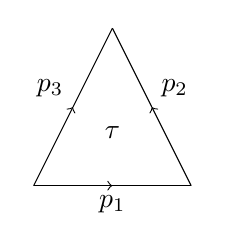
\begin{tikzpicture}
        \draw[->] (-1,0) -- (0, 0) node[below]{$p_1$};
        \draw (0, 0) -- (1, 0);
        \draw[->] (1,0) -- (0.5, 1) node[above right]{$p_2$};
        \draw (0.5, 1) -- (0, 2);
        \draw[->] (-1,0) -- (-0.5, 1) node[above left]{$p_3$};
        \draw (-0.5, 1) -- (0, 2);
        \draw (0, 0.67) node{$\tau$};
    \end{tikzpicture}
\end{figure}

We can continue in this manner with higher-dimensional simplices. Surprise surprise, they form a chain complex: indeed, in the above case
\begin{cd*}
    \R^{\+ T} \arrow[r, "\del"] & \R^{\+ P} \arrow[r, "\del"] & \R^{\+ X}
\end{cd*}
we can see that $\del^2(\tau) = 0$ for all $\tau$, because $p_1 + p_2 - p_3$ is a loop (so its start point minus its end point is zero). We can show something analogous when we consider boundary maps between free modules generated by paths from higher-dimensional simplices as well.

We can thus compute homology as usual:
\begin{align*}
    H_n\of{X; \R} := \quotient{\pker{\del}}{\pim{\del}}
\end{align*}
(and similarly for $H_n\of{X; R}$ where $R$ is any commutative ring).

\subsection{A Formal Definition (of Singular Homology)}

We begin by defining the $n$-simplex.

\begin{boxdefinition}[$n$-Simplex]
    For all $n \in \N$, define the \textbf{$n$-simplex} to be the following subset of $\R^n$:
    \begin{align*}
        \Delta^n := \setst{x \in \R^{n}}{\sum_{i=1}^{n} x_i = 1 \text{ and } \forall i, \ x_i \geq 0}
    \end{align*}
\end{boxdefinition}

Simplices are well-understood, particularly in low dimensions:
\begin{enumerate}
    \item The $0$-simplex is a point.
    \item The $1$-simplex is a line.
    \item The $2$-simplex is a triangle.
    \item The $3$-simplex is a tetrahedron.
\end{enumerate}

\begin{boxdefinition}[Singular $n$-Simplex]
    Let $X$ be a topological space. A continuous map $\sigma : \Delta^n \to X$ is called a \textbf{singular $n$-simplex}.
\end{boxdefinition}

For the remainder of this subsection, let $G$ denote an additively expressed abelian group. Unless otherwise specified, $G$ will denote the integers.

\begin{boxdefinition}[Group of $n$-Chains]
    For all $n \in \N$, define the \textbf{group of $n$-chains $C_n\of{X; G}$} to be the group whose elements are formal finite linear combinations $\sum_{i=1}^{k} \lambda_i \sigma_i$ of singular $n$-simplices $\sigma_i : \Delta^n \to X$ with coefficients $\lambda_i \in G$.
\end{boxdefinition}

Before proceeding any further, we introduce some notation.

\begin{boxnotation}
    We denote by $\brac{v_0, \ldots, \widehat{v_i}, \ldots, v_n}$ the tuple $\brac{v_0, \ldots, v_{i-1}, v_{i+1}, \ldots, v_n}$.
\end{boxnotation}

Now, we define the boundary map.

\begin{boxdefinition}[Boundary Map]
    We let $\partial_n:C_n(X;G)\rightarrow C_{n-1}(X;G)$ denote the ($n^{th}$) \textbf{boundary map}, where $\partial_n$ is defined on a basis of $C_n(X;G)$ by $$\partial_n(\sigma):=\sum_{i=0}^n (-1)^i\sigma\restriction_{[v_0, \ldots, \widehat{v_i}, \ldots, v_n]}$$ where $[v_0, \ldots, v_n]$ is set of vertices of $\triangle^n$ (i.e. standard basis of $\R^n$).
\end{boxdefinition}

The kernel of the boundary map consists of all cycles and the image consists of all boundaries.

\begin{boxlemma}
    $\del_n \circ \del_{n + 1} = 0$.
\end{boxlemma}
\begin{proof}
    Fix $\sigma \in C_n\of{X; G}$. We have
    \begin{align*}
        \del_n\of{\del_{n+1}(\sigma)}
        &= \del_n\of{\sum_{i=0}^{n+1} \parenth{-1}^{i} \cdot \sigma\vert_{\brac{v_0, \ldots, \widehat{v_i}, \ldots, v_{n+1}}}} \\
        &= \sum_{i=0}^{n+1} \sum_{j < i} \parenth{-1}^i \parenth{-1}^j \cdot \sigma\vert_{\brac{v_0, \ldots, \widehat{v_j}, \ldots, \widehat{v_i}, \ldots, v_{n+1}}}
        +
        \sum_{i=0}^{n+1} \sum_{j > i} \parenth{-1}^i \parenth{-1}^{j-1} \cdot \sigma\vert_{\brac{v_0, \ldots, \widehat{v_i}, \ldots, \widehat{v_j}, \ldots, v_{n+1}}} \\
        &= \sum_{i=0}^{n+1} \sum_{j < i} \parenth{-1}^i \parenth{-1}^j \cdot \sigma\vert_{\brac{v_0, \ldots, \widehat{v_j}, \ldots, \widehat{v_i}, \ldots, v_{n+1}}}
        +
        \sum_{j=0}^{n+1} \sum_{i > j} \parenth{-1}^{j} \parenth{-1}^{i-1} \cdot \sigma\vert_{\brac{v_0, \ldots, \widehat{v_j}, \ldots, \widehat{v_i}, \ldots, v_{n+1}}} \\
        &= 0
    \end{align*}
    Thus, $\del_n \circ \del_{n+1} = 0$.
\end{proof}

Thus, $\pim{\del_n} \ssq \pim{\del_{n+1}}$, and the following is a chain complex in the category of abelian groups:
\begin{cd}
    \cdots \arrow[r]
    & C_{n+1}\of{X; G} \arrow[r, "\del_{n+1}"]
    & C_n\of{X; G} \arrow[r, "\del_n"]
    & C_{n-1}\of{X; G} \arrow[r, "\del_{n-1}"]
    & \cdots
    \label{Ch2:CD:Chain_Complex_Cycles}
\end{cd}

\begin{boxdefinition}[Cycles]
    We define a \textbf{cycle} in $C_n\of{X; G}$ to be an element of $\pker{\del_n}$. We denote $Z_n\of{X; G} := \pker{\del_n}$.
\end{boxdefinition}

\begin{boxdefinition}[Boundary Elements]
    We define a \textbf{boundary element} of $C_{n-1}\of{X; G}$ to be an element of $\pim{\del_n}$. We denote $B_n\of{X; G} := \pim{\del_n}$.
\end{boxdefinition}

We are now finally ready to define the $n$th homology group of topological space.

\begin{boxdefinition}[$n$th Homology Group]
    We define the \textbf{$n$th homology group of $X$ with respect to $G$} to be the quotient group
    \begin{align*}
        H_n\of{X; G} := \quotient{\pker{\del_n}}{\pim{\del_{n+1}}} = \quotient{Z_n\of{X;G}}{B_{n+1}\of{X;G}}
    \end{align*}
\end{boxdefinition}

% Note that we can analogously define \textbf{simplicial homology}, where we divide a space into simplices and 

We can also define
\begin{itemize}
    \item \textbf{simplicial homology}, where we divide a space into simplices and proceed geometrically. This coincides with singular homology.
    \item \textbf{reduced homology}, which is exactly the same as singular homology except at index $0$, where we define the boundary map to go from $C_0\of{X; G}$ to $G$ in a way that sends every $\sigma$ to $1$.
\end{itemize}

As we would expect, homology is functorial. As a first step, we show that continuous maps induce morphisms of chain complexes on the chains of cycles. Then, as we know and love, we apply the fact that chain complex morphisms induce homology morphisms.

Moreover, as we would expect, under this correspondence, a homotopy equivalence of topological spaces maps to a homotopy equivalence of chain complexes, which results in an isomorphism on homology.

Finally (as is obvious from functoriality), if we have a homeomorphism, then we get a chain complex isomorphism, and subsequently an isomorphism of homology groups.